\documentclass[tikz,border=4pt]{standalone}
\usepackage[T1]{fontenc}
\usepackage{lmodern}
\usepackage{amsmath}
\usetikzlibrary{positioning,arrows.meta}
% Shared TikZ styles for the Methods workflow figures.
\usepackage{sansmath}
\renewcommand{\familydefault}{\sfdefault}
\sansmath
\newcommand{\step}[2]{\textbf{#1}\\[1pt]{\footnotesize #2}}
\tikzset{
  box/.style={draw, rounded corners=2pt, align=flush center, text width=10.4cm,
              inner sep=5pt, font=\small, line width=0.6pt},
  data/.style={box, draw=black!55, fill=black!6},
  proc/.style={box, draw=blue!55!black, fill=blue!7},
  filt/.style={box, draw=orange!75!black, fill=orange!10},
  result/.style={box, draw=green!45!black, fill=green!8},
  note/.style={align=left, font=\footnotesize\itshape, text=black!70},
  side/.style={box, text width=3.9cm, dashed, draw=black!55, fill=white},
  flow/.style={-{Stealth[length=2.2mm]}, line width=0.7pt, draw=black!65},
}


\begin{document}
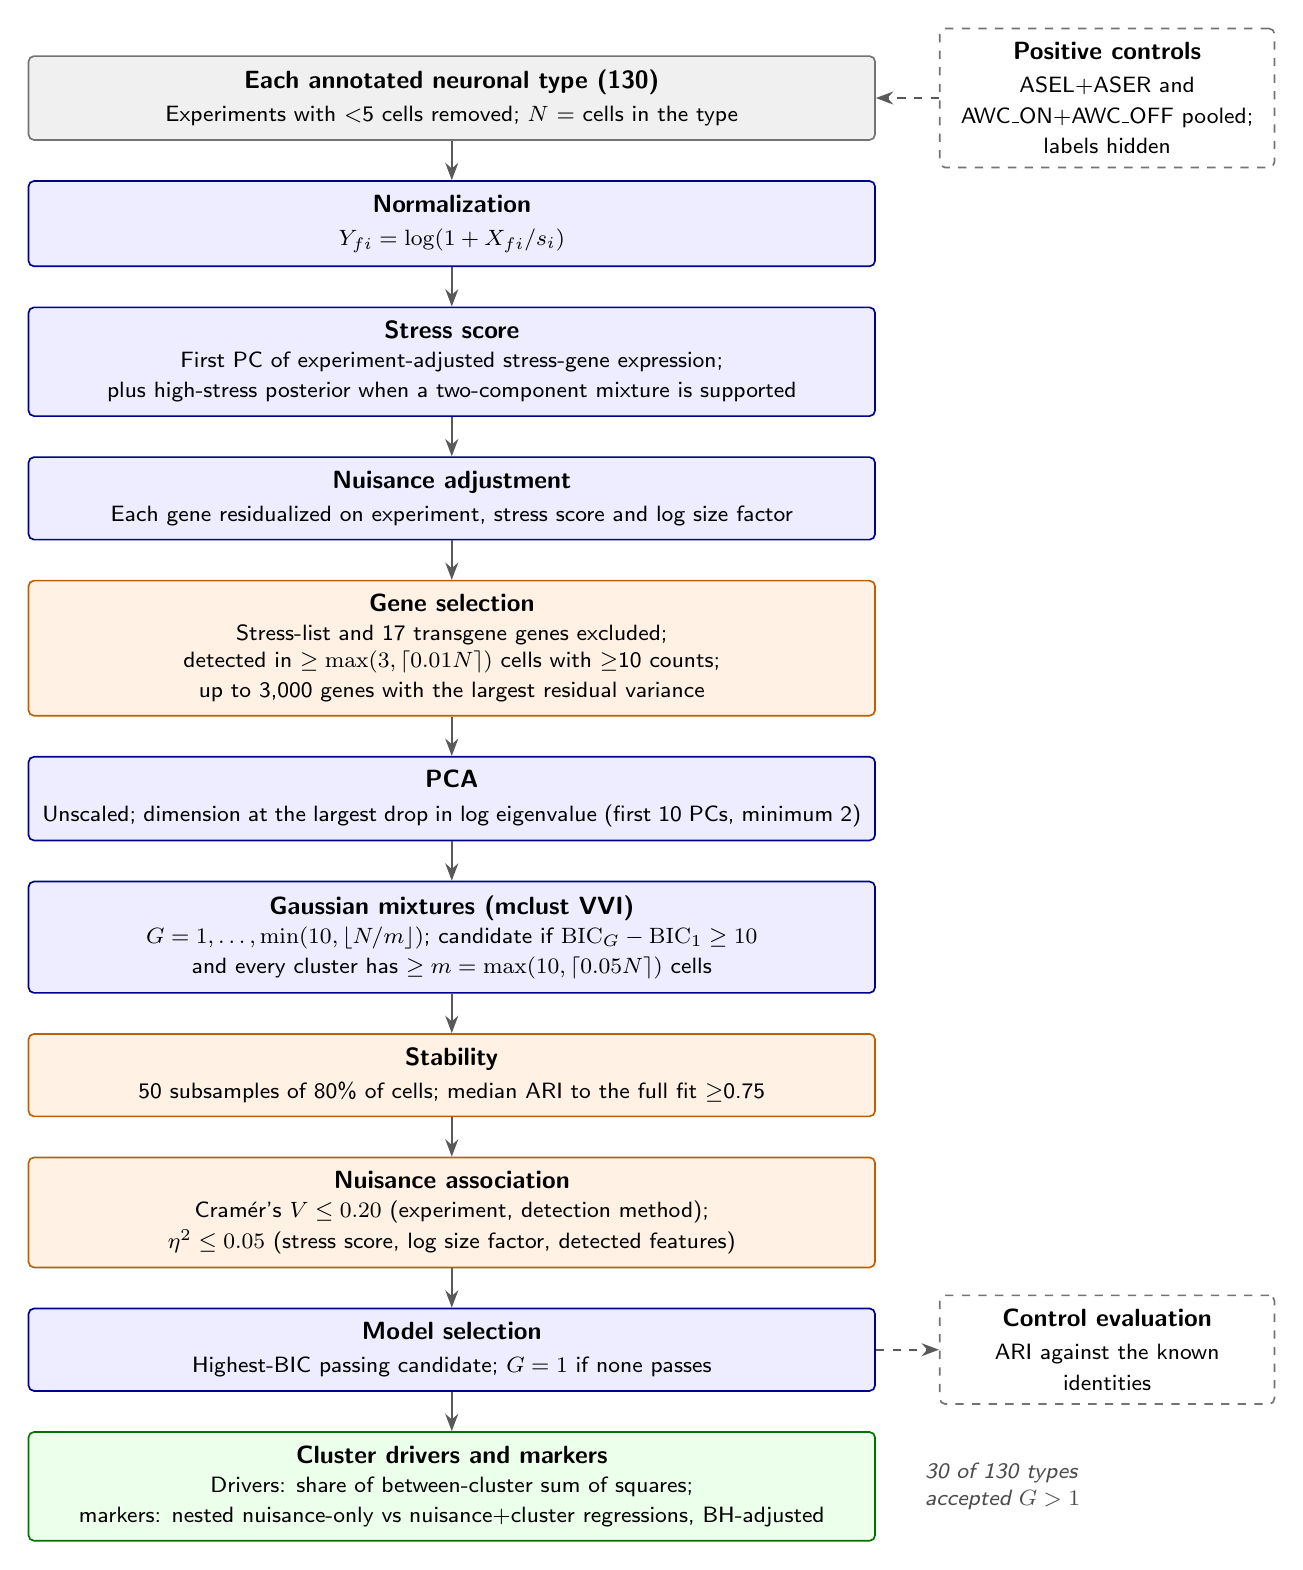
\begin{tikzpicture}[node distance=5mm]
\node[data] (s1) {\step{Each annotated neuronal type (130)}{Experiments with $<$5 cells removed; $N$ = cells in the type}};
\node[proc, below=of s1] (s2) {\step{Normalization}{$Y_{fi}=\log(1+X_{fi}/s_i)$}};
\node[proc, below=of s2] (s3) {\step{Stress score}{First PC of experiment-adjusted stress-gene expression;\\
  plus high-stress posterior when a two-component mixture is supported}};
\node[proc, below=of s3] (s4) {\step{Nuisance adjustment}{Each gene residualized on experiment, stress score and log size factor}};
\node[filt, below=of s4] (s5) {\step{Gene selection}{Stress-list and 17 transgene genes excluded;\\
  detected in $\ge\max(3,\lceil0.01N\rceil)$ cells with $\ge$10 counts;\\
  up to 3,000 genes with the largest residual variance}};
\node[proc, below=of s5] (s6) {\step{PCA}{Unscaled; dimension at the largest drop in log eigenvalue (first 10 PCs, minimum 2)}};
\node[proc, below=of s6] (s7) {\step{Gaussian mixtures (mclust VVI)}{$G=1,\ldots,\min(10,\lfloor N/m\rfloor)$; candidate if $\mathrm{BIC}_G-\mathrm{BIC}_1\ge10$\\
  and every cluster has $\ge m=\max(10,\lceil0.05N\rceil)$ cells}};
\node[filt, below=of s7] (s8) {\step{Stability}{50 subsamples of 80\% of cells; median ARI to the full fit $\ge$0.75}};
\node[filt, below=of s8] (s9) {\step{Nuisance association}{Cram\'er's $V\le0.20$ (experiment, detection method);\\
  $\eta^2\le0.05$ (stress score, log size factor, detected features)}};
\node[proc, below=of s9] (s10) {\step{Model selection}{Highest-BIC passing candidate; $G=1$ if none passes}};
\node[result, below=of s10] (s11) {\step{Cluster drivers and markers}{Drivers: share of between-cluster sum of squares;\\
  markers: nested nuisance-only vs nuisance+cluster regressions, BH-adjusted}};

\foreach \a/\b in {s1/s2,s2/s3,s3/s4,s4/s5,s5/s6,s6/s7,s7/s8,s8/s9,s9/s10,s10/s11} \draw[flow] (\a) -- (\b);

\node[side, right=8mm of s1] (pc) {\step{Positive controls}{ASEL+ASER and AWC\_ON+AWC\_OFF pooled; labels hidden}};
\draw[flow, dashed] (pc) -- (s1);
\node[side, right=8mm of s10] (ari) {\step{Control evaluation}{ARI against the known identities}};
\draw[flow, dashed] (s10) -- (ari);
\node[note, right=of s11] {30 of 130 types\\accepted $G>1$};
\end{tikzpicture}
\end{document}
